\section{Analysis on Weight Difference before and after COVID-situation}

Here our goal is to check if COVID-situation had any impact on weight. We collected data from 230 individuals and we have done the following study depending on that data.

\ 

Consider $(X_{1}, Y_{1})$, .... , $(X_{n}, Y_{n})$ being paired data of $n$-individuals, where

$$X_{1}, .. , X_{n} \ \sim \ \text{IID} \ N(\mu, \sigma^{2}) \ : \ \text{represents weight distribution of $n$-individuals before COVID}$$
$$Y_{1}, .. , Y_{n} \ \sim \ \text{IID} \ N(\mu, \sigma^{2}) \ : \ \text{represents weight distribution of $n$-individuals after COVID}$$

\ 

Here, 
$$E(X_{i}) \ = \ \mu_{1} , \ V(X_{i}) \ = \ \sigma_{1}^{2} , \ \forall \ i \ = \ 1, 2, ... , n$$
$$E(Y_{i}) \ = \ \mu_{2} , \ V(Y_{i}) \ = \ \sigma_{2}^{2} , \ \forall \ i \ = \ 1, 2, ... , n$$
where $\sigma_{1}, \sigma_{2}$ are unknown.

\ 

Assuming normality, we will check if weight remains same before and after COVID against alternative hypothesis or it does not.

\ 

\textbf{Hypothesis}:
$$H_{0} \ : \ \mu_{1} \ = \ \mu_{2} \ \text{vs} \ H_{1} \ : \ \mu_{1} \ \neq \ \mu_{2}$$

\ 

Here, $(X_{i}, Y_{i}) \ \sim \ \text{BVN} \ (\mu_{1}, \ \mu_{2}, \ \sigma_{1}^{2}, \ \sigma_{2}^{2}, \ \rho)$, where $\rho$ being the correlation coefficient of $X_{i}$ and $Y_{i}$.

\ 

Take, 
$$D_{i} \ = \ X_{i} \ - \ Y_{i}, \ \forall \ i \ = \ 1, 2, ... , n$$
$$D_{1}, ..., D_{n} \ \text{are IID} \ N(\mu_{1}, \ \mu_{2}, \ \sigma^{2}), \ \sigma^{2} \ \text{unknown}.$$
where,
$$\sigma^{2} \ = \ V(X) \ + \ V(Y) \ - \ 2 \text{Cov} (X, Y)$$
$$= \ \sigma_{1}^{2} \ + \ \sigma_{2}^{2} \ - \ 2 \rho \sigma_{1} \sigma_{2}$$

\ 

Now, the above test becomes equivalent to one sample test
$$H_{0} \ : \ \mu \ = \ 0 \ \text{vs} \ H_{1} \ : \ \mu \ \neq \ 0 \ \text{with unknown} \ \sigma^{2}$$
where, $\mu \ = \ \mu_{1} \ - \ \mu_{2}$.

\

 In this two-tailed test, consider
 $$\Bar{D} \ = \ \frac{D_{1} \ + ..... + \ D_{n}}{n}$$
 $$E[\Bar{D}] \ = \ E[\frac{D_{1} \ + ..... + \ D_{n}}{n}] \ = \ \frac{n\mu}{n} \ = \ \mu$$
 $$V[\Bar{D}] \ = \ V[\frac{D_{1} \ + ..... + \ D_{n}}{n}] \ = \ \frac{1}{n^{2}} \{ V[D_{1}] \ + ... + \ V[D_{n}] \}$$
 $$= \ \frac{1}{n^{2}} \ n\sigma^{2} \ = \ \frac{\sigma^{2}}{n}, \ \ \text{as \ $D_{1}, ... , D_{n}$, \ are IID}$$

 \ 

 thus, $\Bar{D} \ \sim \ N(\mu, \ \frac{\sigma^{2}}{n})$.

 \ 

 \textbf{Test Statistics}:
Consider following test-statistic using paired t-test.
$$T \ = \ \frac{\Bar{D} \ - \ \mu}{\frac{s}{\sqrt{n}}} , \ \ \text{where $s$ being sample standard-deviation}$$

and $T \ \sim t_{n-1}$, i.e. $t$-distribution with $(n-1)$ degrees of freedom.

\ 

Now, based on our data collected form $n \ = \ 231$ observations :
$$\text{mean} \ = \ \Bar{d} \ = \ 3.058696$$
$$\text{median} \ = \ m_{e} \ = \ 3$$
$$\text{variance} \ = \ 45.643920$$
$$\text{standard deviation} \ = \ 6.756028$$

\ 

Now, under the null-hypothesis $\mu \ = \ 0$ and $s \ = \ 0$,
$$T \ = \ \frac{\Bar{D} \sqrt{n}}{s}$$

using the above data,
$$t \ \approx \ 6.866079, \ \text{observed value of} \ T.$$

\ 

\textbf{Critical Region}:
Since, $n \ = \ 230$ and d.f. $= \ 229$, then
$$T \ \sim \ t_{229, \ 0.975}$$
thus critical region at $5 \%$ level of significance is
$$(-\infty , \ 1.9709] \ \bigcup \ [1.9709, \ \infty).$$

\ 

\textbf{Decision Rule}: To make our decision, we will check if test-statistics lie in confidence interval or not. Our test-statistic is $t \ = \ 6.866079$.\\
If $t$ lies within critical region, we reject null-hypothesis.

\ 

\textbf{Decision}: Since, 
$$t \ = \ 6.866079 \ > \ t_{229, \ 0.975} \ = \ 1.9709$$
i.e. $t$ lies within the critical region $(-\infty , \ 1.9709] \ \bigcup \ [1.9709, \ \infty)$.\\
Therefore, we reject null hypothesis $H_{0} \ : \ \mu \ = \ 0$ against $H_{1} \ : \ \mu \ \neq \ 0$.

\ 

\textbf{Result Interpretation}: Rejecting null-hypothesis provides strong evidence that there is a statistically significant difference in weights before and after COVID-19.

\ 

Hence, our study shows COVID-19 pandemic might had an impact on individual's weight.

\ 

Below, we provide a pictorial representation of our data set of weight difference :

\ 

\begin{figure}[h!]
	\centering
	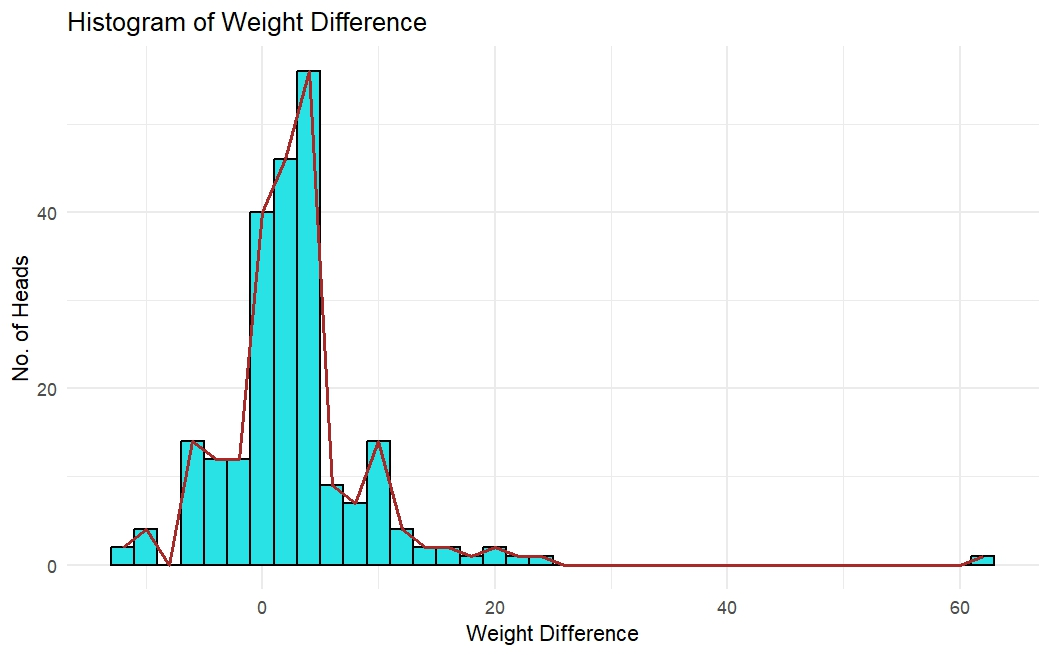
\includegraphics[width=0.7\linewidth]{IMAGES/Image 39.jpg}
	\caption{Difference in Weights}
	\label{G39}
\end{figure}

\ 

We have outliers in our data set. Except these, our data set is clustered between $-20$ to $30$, which indicates persons under study may have encountered significant changes in their weights.

\ 

From the graph above shown (figure \ref{G39}), indicates the mean is greater than zero, which means there is a high probability that individual's had his/her weight decreased after COVID-situation.
